\chapter{Softwares Para Bibliotecas Digitais}
\label{Att:anexobibliotecas}

Nesse anexo estão apresentados os principais produtos de software relacionados a bibliotecas digitais que foram investigados durante o período de preparação do Trabalho de Conclusão de Curso 1.

\section*{Greenstone} 

Greenstone é um conjunto de softwares para a construção e distribuição de coleções de bibliotecas digitais. Ele organiza a informação, publicando-a na Internet ou em CD-ROM. Greenstone é produzido pela Universidade de Waikato, desenvolvido e distribuído em cooperação com a \textit{UNESCO} e a \textit{ONG Human Info}. É um software \textit{open-source}, multilinguagem e emitido nos termos da GNU.
 
O objetivo do software Greenstone é capacitar os usuários, especialmente em universidades, bibliotecas e outras instituições de serviço público, para construir suas próprias bibliotecas digitais. Através de \textit{plugins}, o Greenstone pode importar documentos digitais em formatos de texto incluindo HTML, JPG, TIFF, MP3, PDF, vídeo, Textos, PDF, HTML e documentos similares são convertidos em \textit{Greenstone Archive Format} (GAF), que é um formato XML equivalente.

\section*{KEA}

KEA\footnote{Maiores informações disponíveis em: \url{http://www.nzdl.org/Kea}} é um algoritmo para extração de frases a partir de documentos de texto. Ele pode ser usado para indexação livre ou para a indexação com um vocabulário controlado. Entre outras características, o KEA possui várias versões, é implementado em Java\footnote{Maiores informações em: \url{http://www.java.com}} e é independente de plataforma. Além disso, é um software \textit{open-source} distribuído sob a licença GNU \footnote{Informações em: \url{http://www.gnu.org}}.

No KEA palavras/frases-chave são amplamente utilizadas em grandes coleções de documentos. Elas descrevem o conteúdo dos documentos e fornecem uma espécie de metadados semânticos úteis para uma grande variedade de propósitos. A tarefa de atribuir frases-chave a um documento é chamada de indexação \textit{keyphrase}. Por exemplo, trabalhos acadêmicos são frequentemente acompanhados por um conjunto de frases livremente escolhidas pelo autor. Em bibliotecas, indexadores profissionais selecionam frases-chave de um vocabulário controlado (também chamado \textit{Subject Headings}) de acordo com regras da catalogação definida. Na Internet, bibliotecas digitais, ou qualquer outro depósito de dados também usam frases (\textit{tags} ou etiquetas de conteúdo) para organizar e proporcionar um acesso temático aos seus dados.


\section*{Omeka}
\label{sub:omeka}

Omeka\footnote{Disponível em \url{http://www.omeka.org}} é uma plataforma para disponibilização e manutenção de  bibliotecas digitais bem flexível, isto é, ele se adapta muito bem para sua finalidade, seja ele museu, biblioteca de imagens, livros, lugares (bibliotecas sobre guerras), entre outros. O Omeka é um software livre, com código aberto e escrito em PHP \footnote{Disponível em: \url{http://www.php.net}}. Sua instalação é bastante simples, bastando apenas que a máquina do cliente possua o PHP 5 instalado, juntamente com o banco de dados MySQL\footnote{Disponível em: \url{http://www.mysql.org}} e um servidor HTTP (como o \textit{Apache}\footnote{Informações em: \url{http://www.nginx.org}} ou \textit{nginx}\footnote{Maiores Informações: \url{http://www.nginx.org}}). O Omeka não possui uma finalidade específica como o GreenStone, Dspace, entre outros. Na Figura \ref{fig:finalidadeomeka} podemos visualizar que o Omeka caminha na intersecção de três ferramentas, entre elas: Sistema de gerenciamento de conteúdo (\textit{Web Content Management} ou CMS\footnote{Maiores Informações em: \url{http://pt.wikipedia.org/wiki/Sistema_de_gerenciamento_de_conte\%C3\%BAdo}}), Repositório de arquivos digitais e coleções (biblioteca digital) e sistemas para gerenciamento de museus.

\graphicspath{{figuras/}}
\begin{figure}[H]
\centering
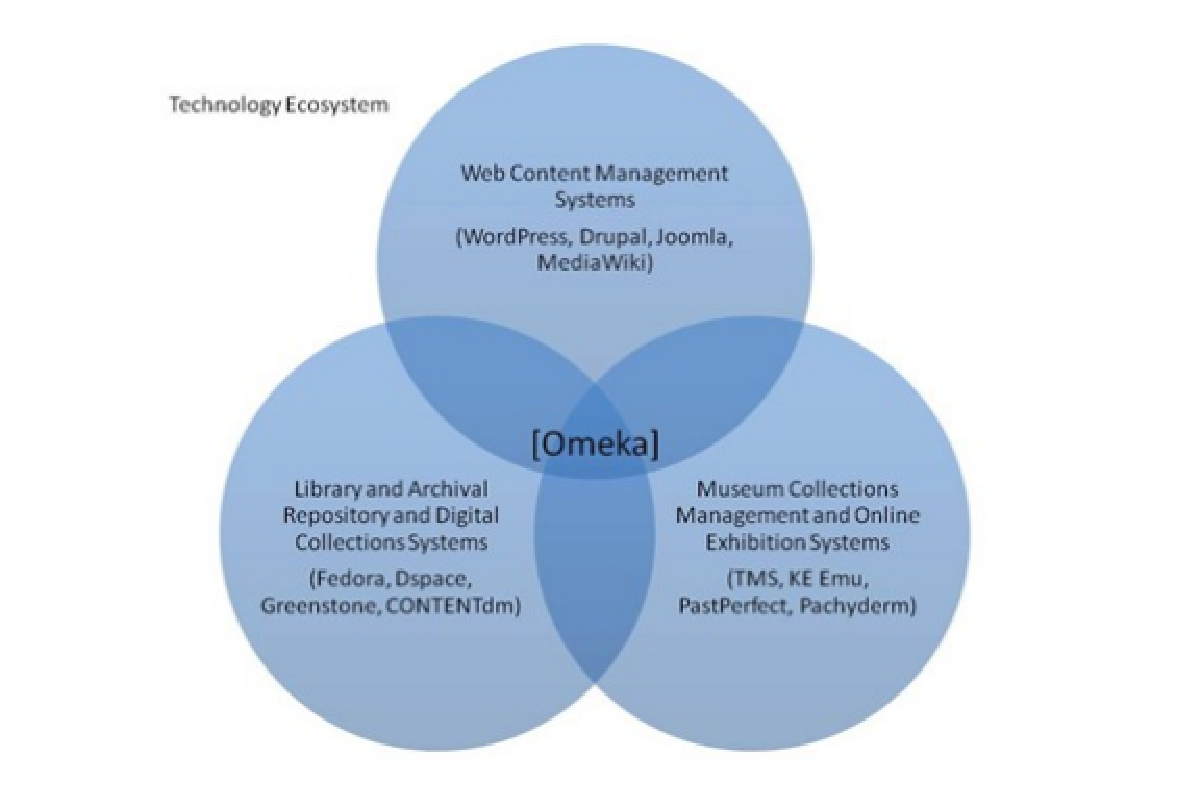
\includegraphics[width=0.7\textwidth]{finalidade_omeka}
\caption[Finalidade do Omeka]{Finalidade do Omeka. Retirado do Site \url{http://www.omeka.org}}
\label{fig:finalidadeomeka}
\end{figure}
%Figura A.2: Finalidade do Omeka Retirado de OMEKA.ORG

O Omeka possui uma interface muito intuitiva e de fácil personalização, isso se deve ao fato de ser construído para pessoas que não são experientes na utilização de computadores. Diferentemente do GreenStone, o Omeka não possui uma interface offline para inserção de dados, já que todas as funções são realizadas dentro do site.

O Omeka possui uma interface muito intuitiva e de fácil personalização, isso se deve ao fato de ser construído para pessoas que não são experientes na utilização de computadores. Diferentemente do GreenStone, o Omeka não possui uma interface offline para inserção de dados, já que todas as funções são realizadas dentro do site. Sua arquitetura possui o padrão MVC (\textit{Model-View-Controller}) que foi visto na seção \ref{sub:arquiteturamvc}.

Outro padrão arquitetural que o Omeka possui é sua extensibilidade. Ou seja, podemos estender temas ou \textit{plugins} desenvolvidos pela comunidade ou por nós, de forma bastante simples: basta colocar o tema dentro da pasta \textit{/themes} (a partir da raiz do Omeka), ou no caso de um \textit{plugin}, existe uma pasta /\textit{plugins}, onde estão localizados todos os \textit{plugins}. Após esse passo, basta logar como administrador na interface do Omeka e ativar os \textit{plugins} ou o tema. Mais detalhes de extensibilidade é visto na seção \ref{sub:arquiteturaplugin}.

Uma das vantagens do desenvolvimento de uma arquitetura extensível através de \textit{plugins} é que novas funcionalidades podem ser incluídas sem a necessidade da interferência do desenvolvedor no código fonte do core do Omeka, uma exemplo de uma nova funcionalidade que foi incluída é a compatibilidade com o protocolo OAI-PMH. Para o desenvolvimento de \textit{plugins} e temas, o Omeka fornece toda uma documentação detalhada para o desenvolvimento.

\section*{Simile}

Símile \footnote{Maiores informações disponíveis em: \url{http://simile.mit.edu}} é um projeto conjunto realizado pelo MIT Libraries~\footnote{Maiores informações em: \url{https://libraries.mit.edu/}}e CSAIL MIT \footnote{Disponível em: \url{http://www.csail.mit.edu/}} visando melhorar a interoperabilidade entre os ativos digitais, esquemas/vocabulários/ontologias, metadados e serviços. Um desafio fundamental é que as coleções que devem interoperar muitas vezes são distribuídas em repositórios individuais, comunitários e institucionais. Ele busca fornecer serviços ao usuário final, com base nos ativos, esquemas/vocabulários/ontologias e metadados realizada em tais repositórios. 

O Simile busca alavancar e estender o DSpace, aumentando o seu apoio a esquemas arbitrários e metadados, principalmente em aplicações de RDF e técnicas da web semântica. O projeto também visa implementar uma arquitetura de difusão digital de ativos baseados em padrões web. A arquitetura de divulgação fornece um mecanismo para adicionar “visões” úteis de um artefato digital particular (ou seja, ativos, esquema ou instância de metadados), e vincular essas opiniões aos serviços de consumo. O projeto está totalmente comprometido com os princípios de código aberto de distribuição de software e de desenvolvimento aberto. Por isso, ele libera a propriedade intelectual criada (software e relatórios) sob uma licença do tipo BSD.
 
\section*{JeromeDL}

JeromeDL\footnote{Disponível em: \url{http://www.jeromedl.org}.}  é uma Biblioteca Digital Semântica Social. Como uma biblioteca digital, permite às instituições facilmente publicarem documentos na web. Ela suporta uma variedade de formatos de documentos e permite armazenar e consultar uma rica descrição bibliográfica de cada documento. Para encontrar documentos relevantes na JeromeDL os usuários podem usar recursos de pesquisa e navegação. O sistema permite a pesquisa por texto completo, por metadados específicos tais como autor ou ano de publicação. Além disso, os usuários também podem encontrar o conteúdo de documentos pela navegação através das categorias de assunto e também por palavras-chave.

Com os serviços do JeromeDL, cada usuário da biblioteca pode marcar livros interessantes, artigos ou outros materiais em diretórios semanticamente anotados. Os usuários podem permitir que outros vejam seus bookmarks e anotações e compartilhar seus conhecimentos dentro de uma rede social. O JeromeDL também pode também tratar um simples recurso de biblioteca como uma postagem de e-mail em um blog. Dessa forma, os usuários podem comentar o conteúdo do recurso e responder aos comentários dos outros e desta forma criar novos conhecimentos.

\section*{DSpace}

DSpace\footnote{Informações adicionais em: \url{http://www.dspace.org/}.} é um software de código fonte aberto que fornece facilidades para o gerenciamento de acervo digital, utilizado para implementação de repositórios institucionais. Suporta uma grande variedade de tipo de documentos, tais como: livros, teses e dissertações, fotografias, filmes, áudio, e outros. Os documentos são organizados em comunidades e coleções.

O DSpace é disponibilizado livremente às instituições de investigação, sob a forma de um produto de código aberto, que pode ser livremente adaptado e expandido funcionalmente, nos termos da BSD \textit{Open source license}. Suas possibilidades de uso incluem: (i) capturar e descrever documentos digitais de acordo com um \textit{workflow} adaptável aos processos específicos de uma comunidade, (ii) distribuir os documentos digitais da instituição na Web, possibilitando a pesquisa e obtenção de cópias aos utilizadores, e (iii) preservar os documentos digitais a longo prazo.

O DSpace aceita todas as formas de materiais digitais, incluindo arquivos de texto, imagem, vídeo e áudio, o que possibilita custodiar os mais variados tipos de conteúdos, tais como, livros, artigos, relatórios técnicos, \textit{working papers}, artigos de conferências, e-teses, conjuntos de dados (estatísticos, geoespaciais, etc.), programas de computador, modelos e simulações visuais, etc. Como forma de se adaptar às necessidades específicas de cada instituição e dos seus departamentos, as possibilidades de “customização” do DSpace incluem, não só, a definição de \textit{workflows “à medida”}, mas também, a especificação de regras de utilização e formatos digitais suportados.

O DSpace permite a aplicação de variadas técnicas que garantam a segurança dos documentos digitais submetidos ao repositório. Algumas destas técnicas consistem na realização de cópias de segurança, espelhamento e atualização da infra-estrutura física (i.e., a migração de um suporte físico obsoleto para outro mais atual). Além disso, a cada item é atribuído um identificador único de forma a assegurar a sua recuperação na ocorrência de uma migração de dados.

O repositório do MIT conta com um mecanismo de aconselhamento aos fornecedores de conteúdos para que a documentação depositada seja fornecida nos formatos mais adequados à sua preservação em longo prazo. Os administradores de cada comunidade têm a possibilidade de limitar o acesso aos conteúdos, quer ao nível do item submetido, quer ao nível da coleção. Para a pesquisa e recuperação dos itens, o processo de submissão de documentos ao DSpace permite a sua descrição usando uma versão qualificada do vocabulário de metadados Dublin Core.

O DSpace foi desenvolvido em linguagem Java e é suportado por um conjunto de ferramentas de código aberto (\textit{open source}), tais como: PostgreSQL\footnote{Informações em: \url{http://www.postgresql.org/}} , Tomcat\footnote{Disponível em: \url{http://tomcat.apache.org/}} e o Lucene (motor de pesquisa)\footnote{Maiores Informações: \url{http://lucene.apache.org/}}. Outros softwares necessários são o Maven\, ant\footnote{Informações em: \url{http://ant.apache.org/}} e ant-optionals\footnote{Maiores infomações em: \url{mvnrepository.com/artifact/ant/ant-optional}}.
